\documentclass[landscape,a0paper,fontscale=0.292]{baposter}

\usepackage[vlined]{algorithm2e}
\usepackage{times}
\usepackage{calc}
\usepackage{url}
\usepackage{graphicx}
\usepackage{amsmath}
\usepackage{amssymb}
\usepackage{relsize}
\usepackage{multirow}
\usepackage{booktabs}

\usepackage{graphicx}
\usepackage{multicol}
\usepackage[T1]{fontenc}
\usepackage{ae}
\usepackage{enumitem}
\setlist[itemize]{nosep}

\usepackage{colortbl}
\usepackage{xcolor}
\usepackage{setspace}
%\usepackage{gensymb} % for \degree
\graphicspath{{images/}}

\setlist[itemize]{leftmargin=*,nosep}
    \setlength{\columnsep}{0.7em}
    \setlength{\columnseprule}{0mm}

\setlist[enumerate]{leftmargin=2.5em,nosep}
    \setlength{\columnsep}{1.0em}
    \setlength{\columnseprule}{0mm}

% %%%%%%%%%%%%%%%%%%%%%%%%%%%%%%%%%%%%%%%%%%%%%%%%%%%%%%%%%%%%%%%%%%%%%%%%%%%%%%%%
% % Save space in lists. Use this after the opening of the list
% %%%%%%%%%%%%%%%%%%%%%%%%%%%%%%%%%%%%%%%%%%%%%%%%%%%%%%%%%%%%%%%%%%%%%%%%%%%%%%%%
% \newcommand{\compresslist}{%
% \setlength{\itemsep}{0pt}%
% \setlength{\itemsep}{0pt}%
% \setlength{\parskip}{0pt}%
% \setlength{\parsep}{0pt}%
% }
\renewcommand{\rmdefault}{ptm} % Arial
\renewcommand{\sfdefault}{ptm} % Arial
\definecolor{purpleheart}{rgb}{0.41, 0.21, 0.61}
\definecolor{purple(html/css)}{rgb}{0.5, 0.0, 0.5}
\newcommand{\headercolor}{white}
\newcommand{\subheadercolor}{black}

%% Network names
\newcommand{\RefineStage}{RefineNet\xspace}
\newcommand{\CoarseStage}{CoarseNet\xspace}
\newcommand{\CoarseStagenospace}{CoarseNet}
\newcommand{\Weightnetwork}{Weight network\xspace}
\newcommand{\weightnetwork}{weight network\xspace}
\newcommand{\Flownetwork}{Flow network\xspace}
\newcommand{\flownetwork}{flow network\xspace}
\newcommand{\featurealignmodule}{deformable alignment module\xspace}
\newcommand{\featurefusionmodule}{temporal attention fusion module\xspace}
\newcommand{\expolowthr}{0.15}
\newcommand{\expohighthr}{0.9}
\newcommand{\SingleStageRefineStage}{RefineNet$^\dag$\xspace}

%% Exposure description
\newcommand{\twoexposure}{two-exposure\xspace}
\newcommand{\threeexposure}{three-exposure\xspace}
\newcommand{\ntwoExposure}{2-Exposure\xspace}
\newcommand{\nthreeExposure}{3-Exposure\xspace}
\newcommand{\lowexposure}{low-exposure\xspace}
\newcommand{\middleexposure}{middle-exposure\xspace}
\newcommand{\highexposure}{high-exposure\xspace}
\newcommand{\LowExposure}{Low-Exposure\xspace}
\newcommand{\MiddleExposure}{Middle-Exposure\xspace}
\newcommand{\HighExposure}{High-Exposure\xspace}
\newcommand{\AllExposure}{All-Exposure\xspace}

\newcommand{\lineardomain}{linear radiance domain\xspace}

% Metrics
\newcommand{\PSNRL}{PSNR-L\xspace}
\newcommand{\PSNRT}{PSNR\xspace}
\newcommand{\SSIMT}{SSIM-T\xspace}
\newcommand{\VQM}{HDR-VQM\xspace}
\newcommand{\VDP}{HDR-VDP2\xspace}

% Mathematical variables
\newcommand{\crf}{\mathcal{F}}
\newcommand{\hdr}{H}
\newcommand{\tmhdr}{T}
\newcommand{\gttmhdr}{\tilde{\tmhdr}}
\newcommand{\ldr}{L}
\newcommand{\lhdr}{I}
\newcommand{\originldr}{\tilde{\ldr}}
%\newcommand{\hdrtoldr}{l}
\newcommand{\ldrtohdr}{h}
\newcommand{\hdrtoldr}{g}
\newcommand{\expt}{t}
\newcommand{\flow}{F}
\newcommand{\warpldr}{\hat{L}}
\newcommand{\warplhdr}{\hat{I}}
\newcommand{\weight}{\omega}
\newcommand{\coarsehdr}{\hdr^c}
\newcommand{\coarsetmhdr}{\tmhdr^c}
\newcommand{\coarseloss}{\mathcal{L}^\text{c}}
\newcommand{\refinehdr}{\hdr^r}
\newcommand{\refinetmhdr}{\tmhdr^r}
\newcommand{\finalhdr}{\hdr}
\newcommand{\finaltmhdr}{\tmhdr}
\newcommand{\refineloss}{\mathcal{L}^r}
\newcommand{\totalloss}{\mathcal{L}}
\newcommand{\validmask}{M}
\newcommand{\feature}{F}
\newcommand{\alignedfeature}{\tilde{F}}

% Datasets
\newcommand{\staticdatalong}{\emph{static scenes with GT}\xspace}
\newcommand{\staticdataWithMotion}{\emph{static scenes} augmented with random global motion\xspace}
\newcommand{\dynamicgtdatalong}{\emph{dynamic scenes with GT}\xspace}
\newcommand{\dynamicdatalong}{\emph{dynamic scenes without GT}\xspace}
\newcommand{\staticdata}{$\mathcal{D}_s^{gt}$\xspace}
\newcommand{\dynamicgtdata}{$\mathcal{D}_d^{gt}$\xspace}
\newcommand{\dynamicdata}{$\mathcal{D}_d$\xspace}
\newcommand{\kalantaridata}{\emph{Kalantari13} dataset\xspace}
\newcommand{\traindataHDR}{$D_\text{HDR}$\xspace}
\newcommand{\traindataVimeo}{$D_\text{Vimeo}$\xspace}

\newcommand{\NumOfStaticTwoExp}{49}
\newcommand{\NumOfStaticThreeExp}{48}
\newcommand{\NumOfDynamicGTTwoExp}{76}
\newcommand{\NumOfDynamicGTThreeExp}{108}
\newcommand{\NumOfDynamicTwoExp}{37}
\newcommand{\NumOfDynamicThreeExp}{38}

\newcommand{\pokerscene}{\scene{Poker Fullshot}}
\newcommand{\carouselscene}{\scene{Carousel Fireworks}}
\newcommand{\ThrowTowelScene}{\scene{Throwing Towel 2Exp}}
\newcommand{\NinjaScene}{\scene{Ninja 2Exp}}
\newcommand{\FireScene}{\scene{Fire 2Exp}}
\newcommand{\CleaningScene}{\scene{Cleanining 3Exp}}
\newcommand{\DogScene}{\scene{Dog 3Exp}}
\newcommand{\EmailScene}{\scene{Checking Email 3Exp}}

% Methods
\newcommand{\YanCVPR}{Yan19~\cite{yan2019attention}\xspace}
\newcommand{\KalantariTOG}{Kalantari13~\cite{kalantari2013patch}\xspace}
\newcommand{\KalantariEG}{Kalantari19~\cite{kalantari2019deep}\xspace}

%%%%%%%%%%%%%%%%%%%%%%%%%%%%%%%%%%%%%%%%%%%%%%%%%%%%%%%%%%%%%%%%%%%%%%%%%%%%%
%% Begin of Document
%%%%%%%%%%%%%%%%%%%%%%%%%%%%%%%%%%%%%%%%%%%%%%%%%%%%%%%%%%%%%%%%%%%%%%%%%%%%%
\begin{document}
%%%%%%%%%%%%%%%%%%%%%%%%%%%%%%%%%%%%%%%%%%%%%%%%%%%%%%%%%%%%%%%%%%%%%%%%%%%%%
%% Here starts the poster
%%---------------------------------------------------------------------------
%% Format it to your taste with the options
%%%%%%%%%%%%%%%%%%%%%%%%%%%%%%%%%%%%%%%%%%%%%%%%%%%%%%%%%%%%%%%%%%%%%%%%%%%%%
\begin{poster}{
    % Show grid to help with alignment
    grid=false,
    columns=5,
    % Column spacing
    colspacing=0.7em,
    % Color style
    headerColorOne=purple(html/css),
    borderColor=purple(html/css),
    %headerColorOne=purpleheart,
    %borderColor=purpleheart,
    %headerColorOne=cyan!20!white!90!black,
    %borderColor=cyan!30!white!90!black,
    % Format of textbox
    textborder=faded,
    % Format of text header
    headerborder=open,
    headershape=roundedright,
    headershade=plain,
    background=none,
    bgColorOne=cyan!10!white,
    headerheight=0.12\textheight
}
% Eye Catcher
{
    
\includegraphics[height=0.045\linewidth]{logo/HKU_logo}
    \makebox[0.005\textwidth]{} 
    \raisebox{0.00\height}{
\includegraphics[height=0.045\linewidth]{logo/alibaba.png}}
    \makebox[0.005\textwidth]{} 
    \raisebox{0.00\height}{
\includegraphics[height=0.045\linewidth]{logo/PolyU.svg.png}}
}
% Title
{
    \sc\Large\bf HDR Video Reconstruction: A Coarse-to-fine Network and A Real-world Benchmark Dataset
}
% Authors
{
    {\large Guanying Chen$^{1,2}$ \quad Chaofeng Chen$^{1}$ \quad Shi Guo$^{2,3}$ \quad Zhetong Liang$^{2,3}$ \quad Kwan-Yee K. Wong$^1$ \quad Lei Zhang$^{2,3}$} \\
    {{\normalsize $^1$Department of Computer Science, The University of Hong Kong} \quad
    {\normalsize $^2$DAMO Academy, Alibaba Group} \quad \\
    {\normalsize $^3$Department of Computing, The Hong Kong Polytechnic University}}
}
% University logo
{
    \begin{tabular}{c}
        \raisebox{-1.0\height}{
\includegraphics[width=0.15\linewidth]{logo/ICCV21_logo.png}}\\
        \raisebox{-0.7\height}{
\includegraphics[width=0.15\linewidth]{images/qrcode.pdf}}
    \end{tabular}
}

%%%%%%%%%%%%%%%%%%%%%%%%%%%%%%%%%%%%%%%%%%%%%%%%%%%%%%%%%%%%%%%%%%%%%%%%%%%%%%
%%% Now define the boxes that make up the poster
%%%---------------------------------------------------------------------------
%%% Each box has a name and can be placed absolutely or relatively.
%%% The only inconvenience is that you can only specify a relative position 
%%% towards an already declared box. So if you have a box attached to the 
%%% bottom, one to the top and a third one which should be inbetween, you 
%%% have to specify the top and bottom boxes before you specify the middle 
%%% box.
%%%%%%%%%%%%%%%%%%%%%%%%%%%%%%%%%%%%%%%%%%%%%%%%%%%%%%%%%%%%%%%%%%%%%%%%%%%%%%

%%%%%%%%%%%%%%%%%%%%%%%%%%%%%%%%%%%%%%%%%%%%%%%%%%%%%%%%%%%%%%%%%%%%%%%%%%%%%%
\headerbox{\bf\color{\headercolor} Problem and Contribution}{name=contribution,column=0,row=0,span=2}{
    \begin{minipage}[c]{0.48\linewidth}
        \textbf{\color{\subheadercolor}Goal:} Introducing a coarse-to-fine framework and a real-world video dataset for HDR video reconstruction from sequences with alternating exposures.
    \end{minipage}
    \hfill
    \begin{minipage}[c]{0.48\linewidth}
        \begin{center}
            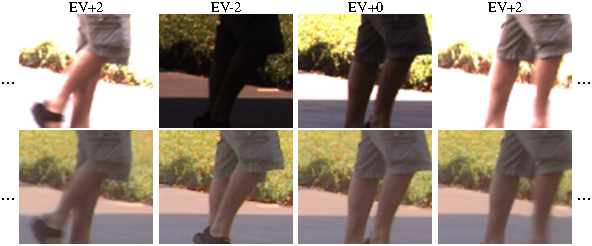
\includegraphics[width=\textwidth]{images/teaser-crop}
        \end{center}
    \end{minipage}

    \textbf{\color{\subheadercolor}Contributions:}
    \begin{itemize}
        \item We propose a two-stage framework, which first performs image alignment and HDR fusion in the image space and then in feature space, for HDR video reconstruction from sequences with alternating exposures.
        \item We create a real-world video dataset captured with alternating exposures as a benchmark to enable quantitative evaluation for this problem. 
    \end{itemize}  
    
}

\headerbox{\bf\color{\headercolor} The Proposed Coarse-to-fine Network}{name=abstract,column=0,below=contribution,span=2}{

    \textbf{\color{\subheadercolor}Input Preprocessing}

    \begin{itemize}
        \item {\scriptsize We replace the CRF of the input images with a fixed gamma curve as $\ldr_i = (\crf^{-1} (\originldr_i))^{1/\gamma}$, where $\gamma=2.2$} \vspace{-0.2em}
        \item {\scriptsize Global alignment is then performed using a similarity transformation to compensate camera motions among neighboring frames}
    \end{itemize}

    \vspace{0.2em}
    \textbf{\color{\subheadercolor}Network Architecture for Two Alternating Exposures:} 
    \vspace{-0.5em}
    \begin{center}
        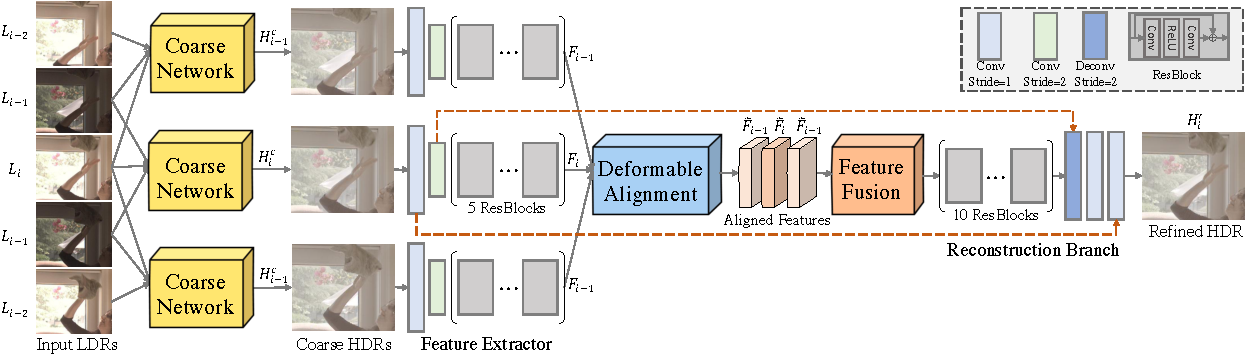
\includegraphics[width=0.95\textwidth]{images/network-crop.pdf}
    \end{center}

    \vspace{-0.7em}
    \textbf{\color{\subheadercolor}CoarseNet Performs Alignment and Fusion in Image Space:}

    \begin{itemize}
        \item {\scriptsize CoarseNet warps neighboring frames to the center frame using optical flows, and reconstructs the HDR image by pixel blending}
    \end{itemize}
    
    \vspace{0.2em}
    \begin{minipage}[c]{0.48\linewidth}
        \begin{center}
            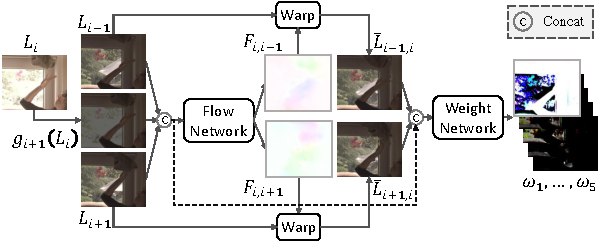
\includegraphics[width=\textwidth]{images/coarsenet-crop.pdf}
        \end{center}
    \end{minipage}
    \hfill
    \begin{minipage}[c]{0.48\linewidth}
        \vspace{0.2em}
        \textbf{\footnotesize Coarse HDR Reconstruction:}
        \begin{equation}
            \tiny
            \label{eq:weighted_sum}
            \coarsehdr_i = \frac{\weight_1 \lhdr_{i-1} + \weight_2 \warplhdr_{i-1,i} + \weight_3 \lhdr_i + \weight_4 \warplhdr_{i+1,i} + \weight_5 \lhdr_{i+1}}{\sum_{k=1}^5 \weight_k}.
        \end{equation}
        \textbf{\footnotesize Loss Function ($L_1$ loss):}
        \begin{equation}
            \label{eq:mutonemap}
            \tiny
            \coarseloss = \parallel \coarsetmhdr_i - \gttmhdr_i \parallel_1, \quad  \coarsetmhdr_i = \frac{\log(1+\mu \coarsehdr_i)}{\log(1+\mu)}
        \end{equation}
    \end{minipage}

    \vspace{0.5em}
    \textbf{\color{\subheadercolor}RefineNet Performs Alignment and Fusion in Feature Space:}

    %\vspace{0.2em}
    \begin{itemize}
        \item {\scriptsize Features of neighboring frames are aligned to the center frame using deformable alignment module} \vspace{-0.2em}
        \item {\scriptsize The aligned feature is fused with a temporal attention for HDR reconstruction}
    \end{itemize}

    \vspace{0.5em}
    \begin{minipage}[c]{0.48\linewidth}
        \begin{center}
            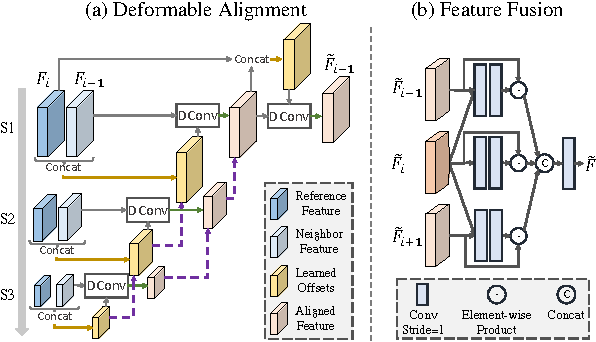
\includegraphics[width=0.9\textwidth]{images/deformable_fusion_module-crop.pdf}
        \end{center}
    \end{minipage}
    \hfill
    \begin{minipage}[c]{0.48\linewidth}
        \textbf{\footnotesize Refined HDR Reconstruction:}

        \begin{minipage}[c]{0.48\linewidth}
            \begin{equation}
                \label{eq:hdr_merge}
                \tiny
                \finalhdr_i = \validmask_i \odot \coarsehdr_i + (1 - \validmask_i) \odot \refinehdr_i
            \end{equation}
        \end{minipage}
        \hfill
        \begin{minipage}[c]{0.48\linewidth}
            \vspace{1em}
            \begin{center}
                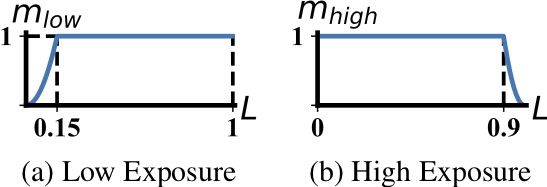
\includegraphics[width=\textwidth]{images/blend_curve-crop.jpg}
            \end{center}
        \end{minipage}

        \vspace{1.0em} 
        \textbf{\footnotesize Loss function ($L_1$ and perceptual loss):}
        \begin{equation}
            \tiny
            \refineloss = \, \frac{\parallel \finaltmhdr_i - \gttmhdr_i \parallel_1}{\parallel 1 - \validmask_i \parallel_1} + \sum\nolimits_k \parallel \phi_k(\tmhdr_i) - \phi_k(\gttmhdr_i) \parallel_1
        \end{equation}
    \end{minipage}


}
%
\headerbox{\bf\color{\headercolor} The Introduced Real-world Video Dataset}{name=dataset,column=2,row=0,span=3}{
    \begin{minipage}[t]{0.44\linewidth}
        \textbf{\color{\subheadercolor}Dataset Statistics}
        \vspace{-0.5em}
        \begin{center}
            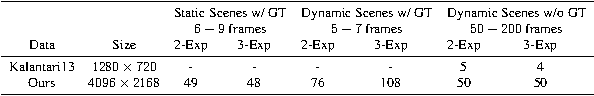
\includegraphics[width=0.9\textwidth]{images/real_data_stats-crop.pdf}
        \end{center}
        \vspace{-1em}
        \textbf{\color{\subheadercolor}Samples in Static Scenes With GT}
        \vspace{-0.6em}
        \begin{center}
            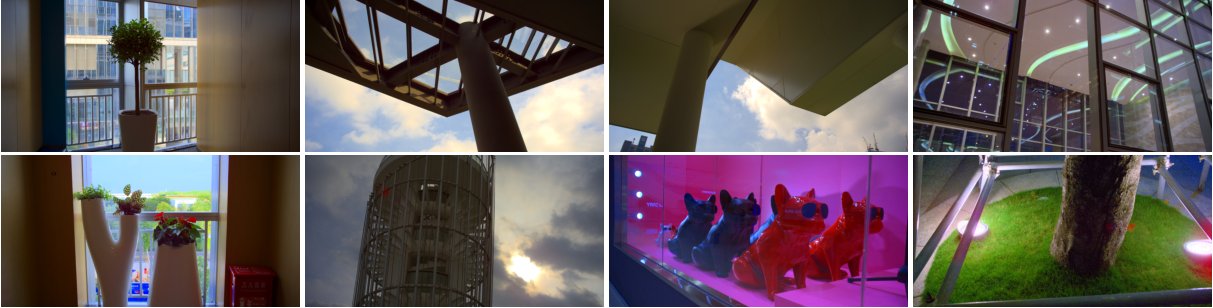
\includegraphics[width=0.78\textwidth]{images/static_samples-crop.pdf}
        \end{center}
        \vspace{-1em}
        \textbf{\color{\subheadercolor}Samples in Dynamic Scenes Without GT}
        \vspace{-0.7em}
        \begin{center}
            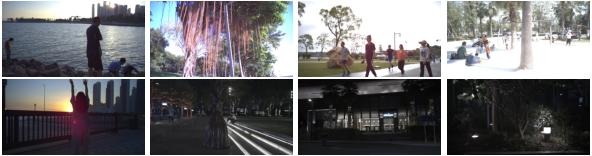
\includegraphics[width=0.78\textwidth]{images/dynamic_nogt_samples-crop.pdf}
        \end{center}
    \end{minipage}
    \hfill
    \begin{minipage}[t]{0.54\linewidth}
        \textbf{\color{\subheadercolor}Generating the LDRs-HDR Pairs for Dynamic Scenes with GT}

        {\scriptsize Row 1: the selected image sequence.\\[-0.5em]
            Rows 2 and 3: two sample pairs with low-exposure and high-exposure reference frames, respectively.}
        \vspace{-0.7em}
        \begin{center}
            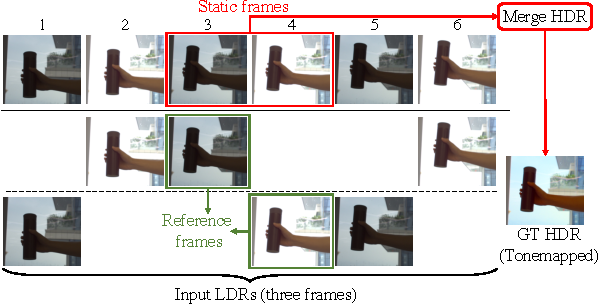
\includegraphics[width=0.77\textwidth]{images/dynamic_gt_preparation-crop.pdf}
        \end{center}
        \vspace{-0.7em}
        \begin{enumerate}
            \scriptsize
            \item The subject is asked to keep still for 2s, an HDR image is generated for this static frame
            \item The subject is asked to move back-and-forth (e.g., waving hands or walking)
            \item Select a sequence whose center frame was the static frame, and arrange it to be proper pairs 
        \end{enumerate}
    \end{minipage}

}
\headerbox{\bf\color{\headercolor} Experiments \& Results}{name=results,column=2,below=dataset,span=3}{
    \begin{minipage}[t]{0.30\linewidth}
        \textbf{\color{\subheadercolor}Quantitative Results on Synthetic Data}
        %\vspace{-0.8em}
        \begin{center}
            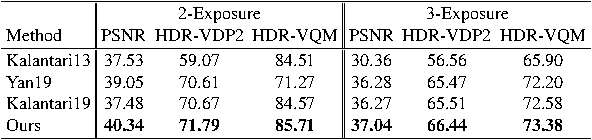
\includegraphics[width=\textwidth]{images/res_quant_syn-crop.pdf}
        \end{center}
    \end{minipage}
    \hfill
    \begin{minipage}[t]{0.30\linewidth}
        \textbf{\color{\subheadercolor}Qualitative Results on Synthetic Data}
        \vspace{-0.8em}
        \begin{center}
            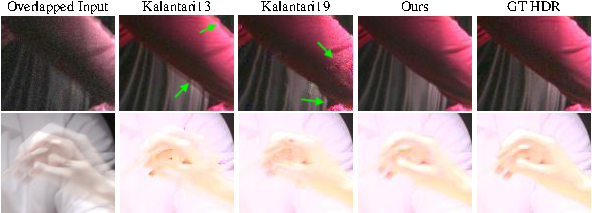
\includegraphics[width=\textwidth]{images/res_qual_syn-crop.pdf}
        \end{center}
    \end{minipage}
    \hfill
    \begin{minipage}[t]{0.32\linewidth}
        \textbf{\color{\subheadercolor}Qualitative Results on Real Static Data}
        \vspace{-0.8em}
        \begin{center}
            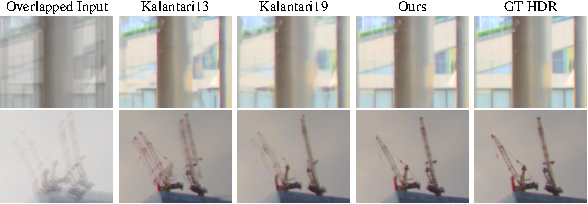
\includegraphics[width=0.97\textwidth]{images/res_qual_real_static-crop.pdf}
        \end{center}
    \end{minipage}

    \vspace{0.2em}
    \begin{minipage}[c]{0.65\linewidth}
        \textbf{\color{\subheadercolor}Quantitative Results on the Introduced Real-world Dataset}
        \vspace{-0.8em}
        \begin{center}
            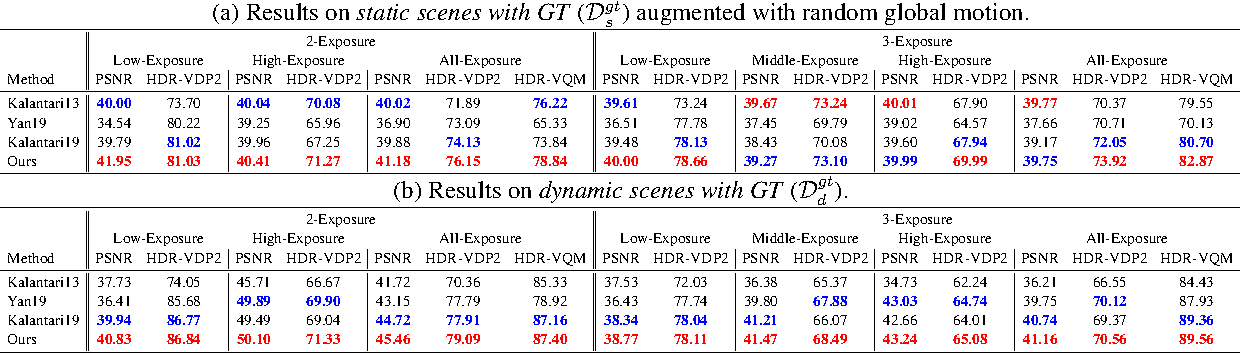
\includegraphics[width=\textwidth]{images/res_quant_real-crop.pdf}
        \end{center}
    \end{minipage}
    \hfill
    \begin{minipage}[c]{0.34\linewidth}
        \textbf{\color{\subheadercolor}Qualitative Results on Real Dynamic Data}
        \begin{center}
            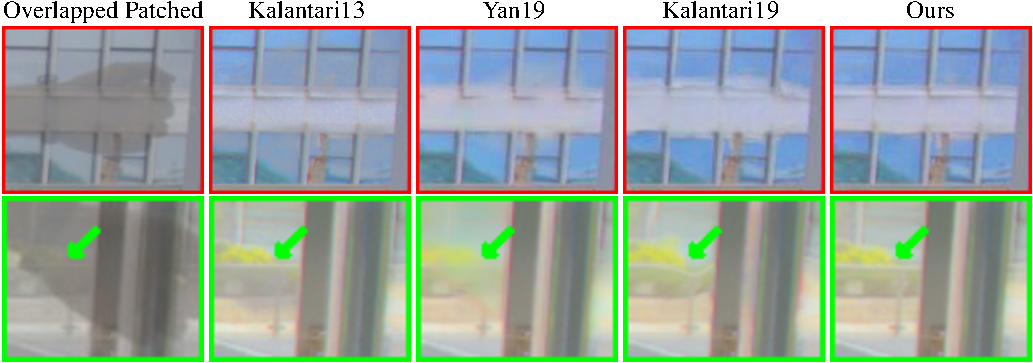
\includegraphics[width=\textwidth]{images/res_qual_real_dynamic-crop.pdf}
        \end{center}
    \end{minipage}

    \vspace{0.3em}
    \begin{minipage}[t]{0.65\linewidth}
        \textbf{\color{\subheadercolor}Visual Comparison on THROWING TOWEL Scene from Kalantari13 Dataset}
        \vspace{-0.8em}
        \begin{center}
            \includegraphics[width=\textwidth]{images/res_qual_TOG13-crop.pdf}
        \end{center}
    \end{minipage}
    \hfill
    \begin{minipage}[t]{0.34\linewidth}
        \textbf{\color{\subheadercolor}Model Parameter and Runtime:}
        \vspace{-0.4em}
        \begin{center}
            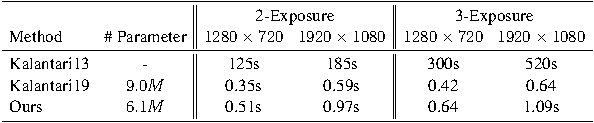
\includegraphics[width=\textwidth]{images/runtime-crop.pdf}
        \end{center}
        
        \vspace{-0.5em}
        \textbf{\color{\subheadercolor}Ablation Study:}
        \vspace{-0.5em}
        \begin{center}
            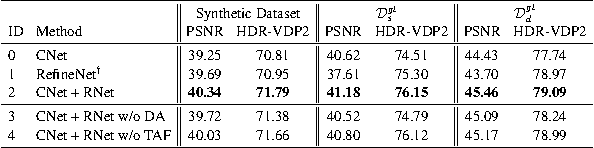
\includegraphics[width=\textwidth]{images/ablation_study-crop.pdf}
        \end{center}

        \vspace{-0.5em}
        \textbf{\color{\headercolor}References:}
        \begin{enumerate}[leftmargin=*,label={[\arabic*]}]
            \tiny
            \item Kalantari13: Patch-based high dynamic range video, TOG 2013
            \item Yan19: Attention- guided network for ghost-free high dynamic range imaging, CVPR 2019
            \item Kalantari19: Deep HDR video from sequences with alternating exposures. Computer Graphics Forum, 2019
        \end{enumerate}
    \end{minipage}
    
}

\end{poster}
\end{document}
